
\subsection{Diseño}


\begin{itemize}
  \item \textbf{Diagrama Entidad - Relación:}

En la figura \ref{fig:er_lugar}, se observa el diagrama Entidad - Relación correspondiente a los \emph{lugares} dentro del campus Universitario.

\begin{figure}[H]
  \begin{center}
    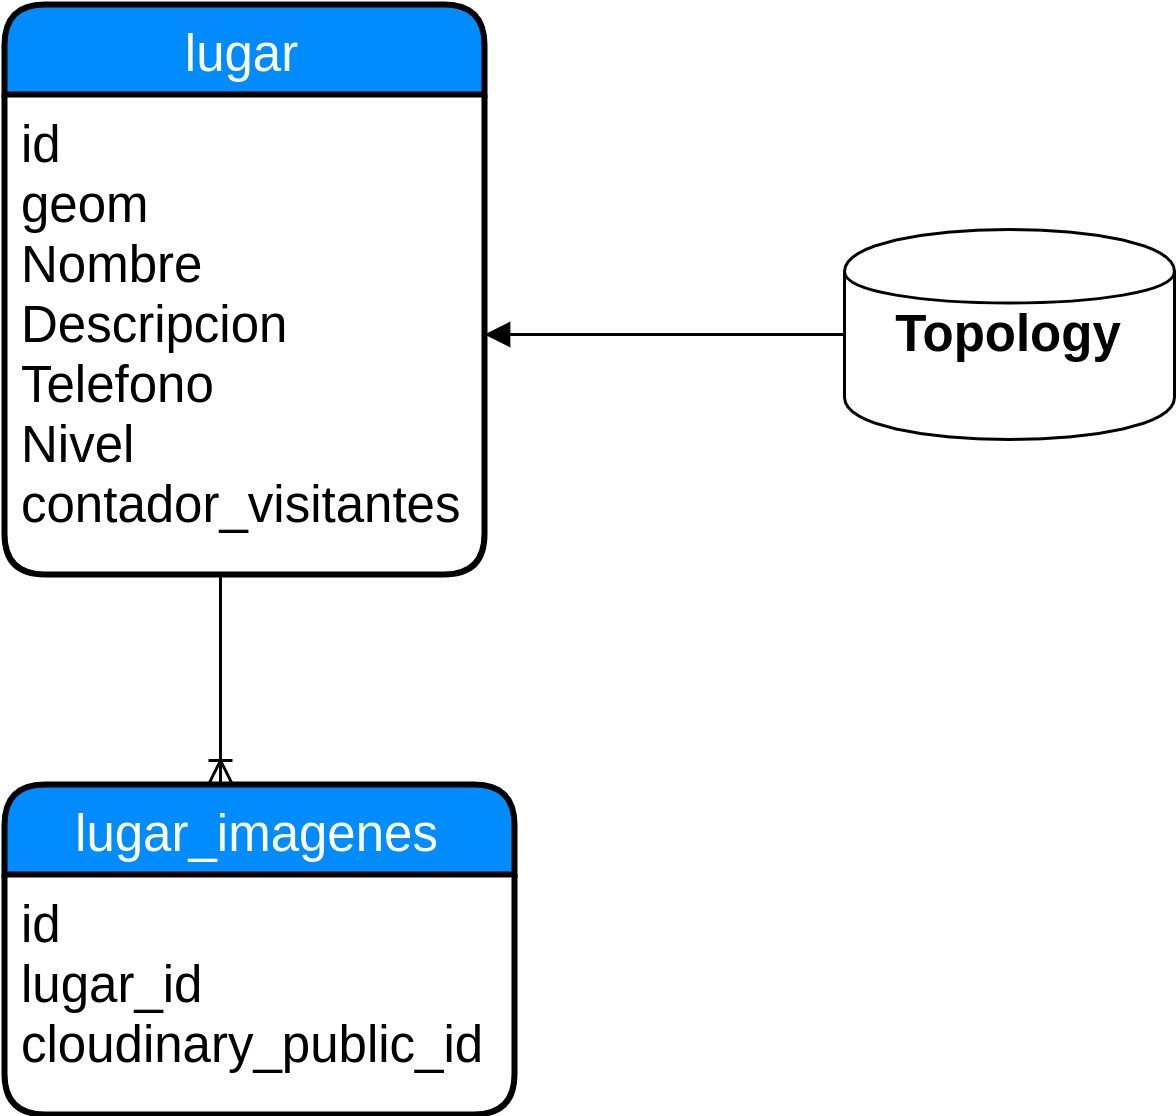
\includegraphics[width=0.4\textwidth]{diagramas/er_lugar}
  \end{center}
  \caption{Diagrama ER: Lugares}
  \label{fig:er_lugar}
  \caption*{Fuente: Elaboración propia}
\end{figure}



\item \textbf{Diagrama de Secuencia:}

En la figura \ref{fig:sequence_ver_lugar}, se observa el diagrama de secuencia correspondiente obtención de la lista e información de lugares.


\begin{figure}[H]
  \begin{center}
    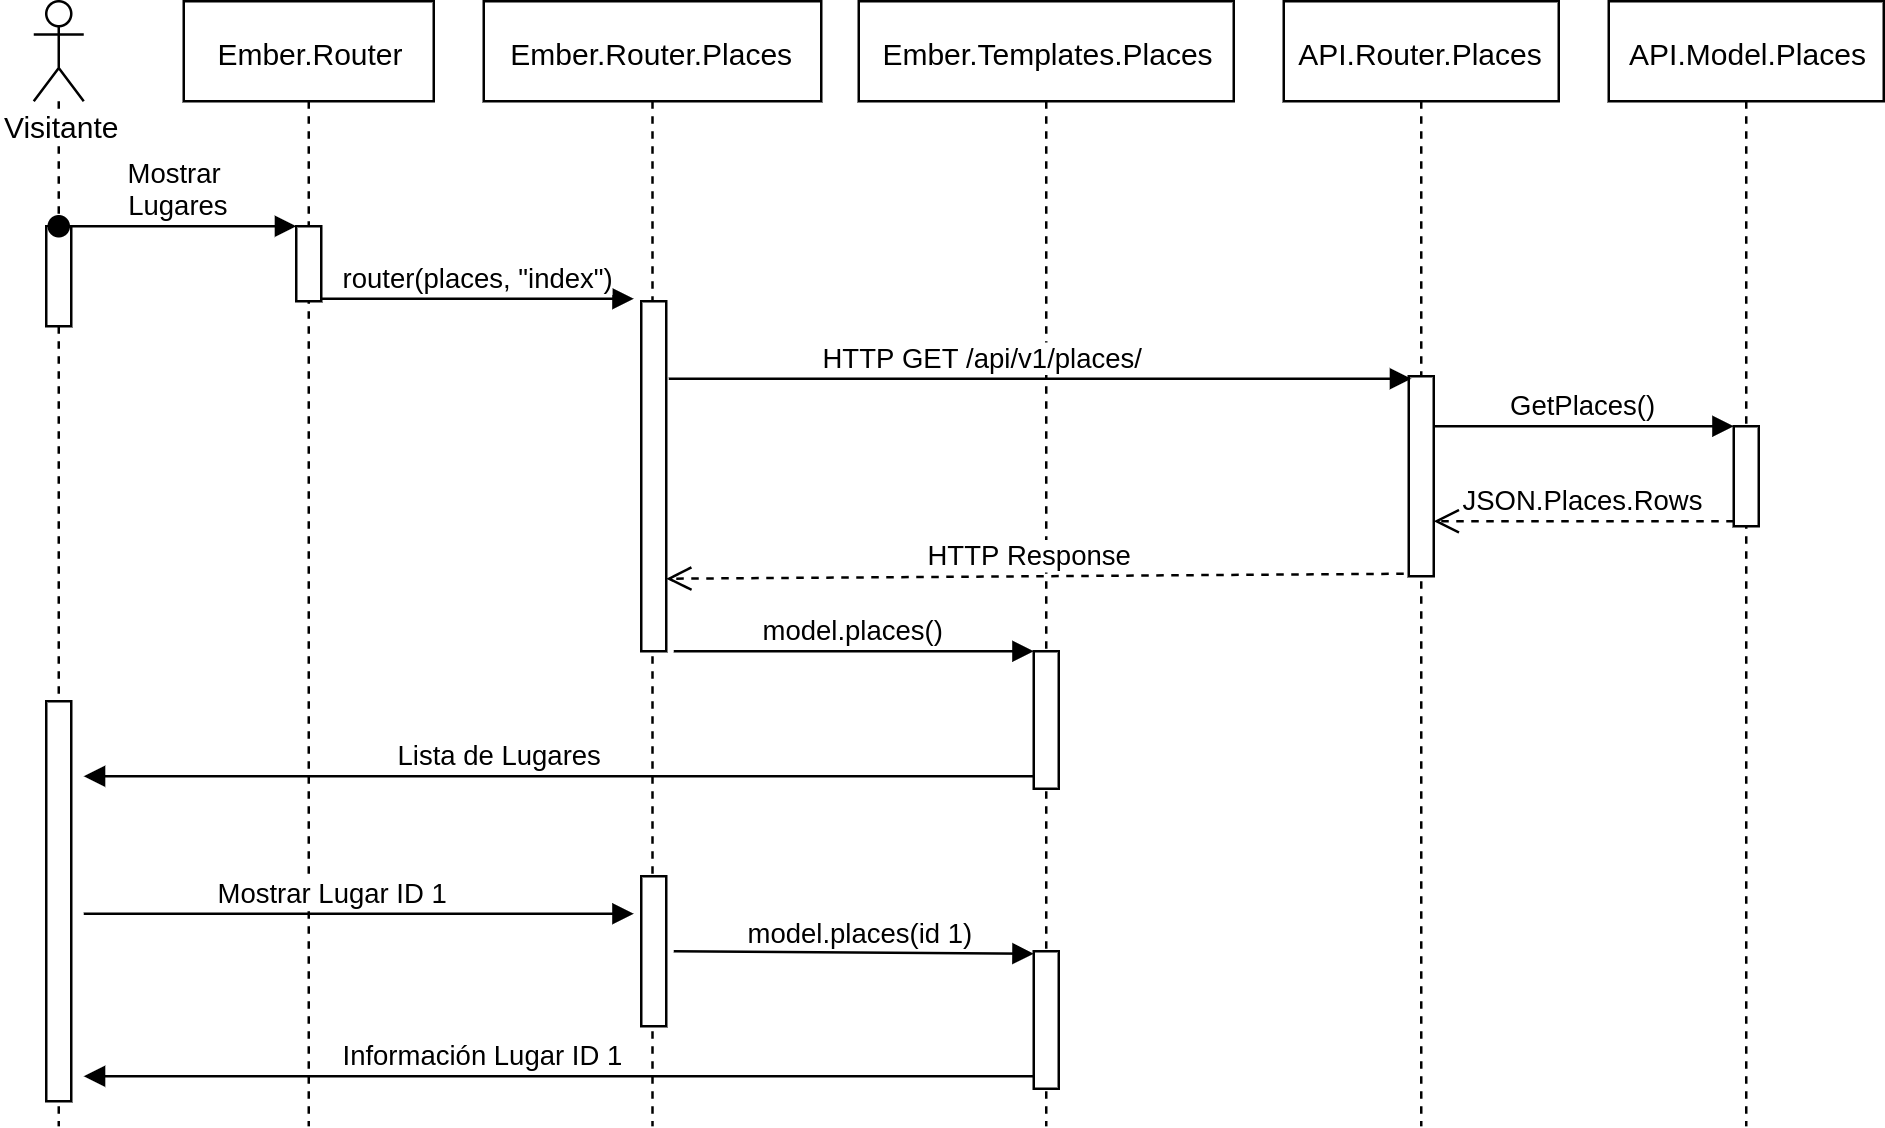
\includegraphics[width=0.9\textwidth]{diagramas/sequence_ver_lugar}
  \end{center}
  \caption{Diagrama de Secuencia: Lista e Información de Lugares}
  \label{fig:sequence_ver_lugar}
  \caption*{Fuente: Elaboración propia}
\end{figure}



\item \textbf{Diagrama de Clases:}


En la figura \ref{fig:clases_lugares}, se observa el diagrama de clases correspondiente a los lugares y la información de estos.

\begin{figure}[H]
\begin{center}
  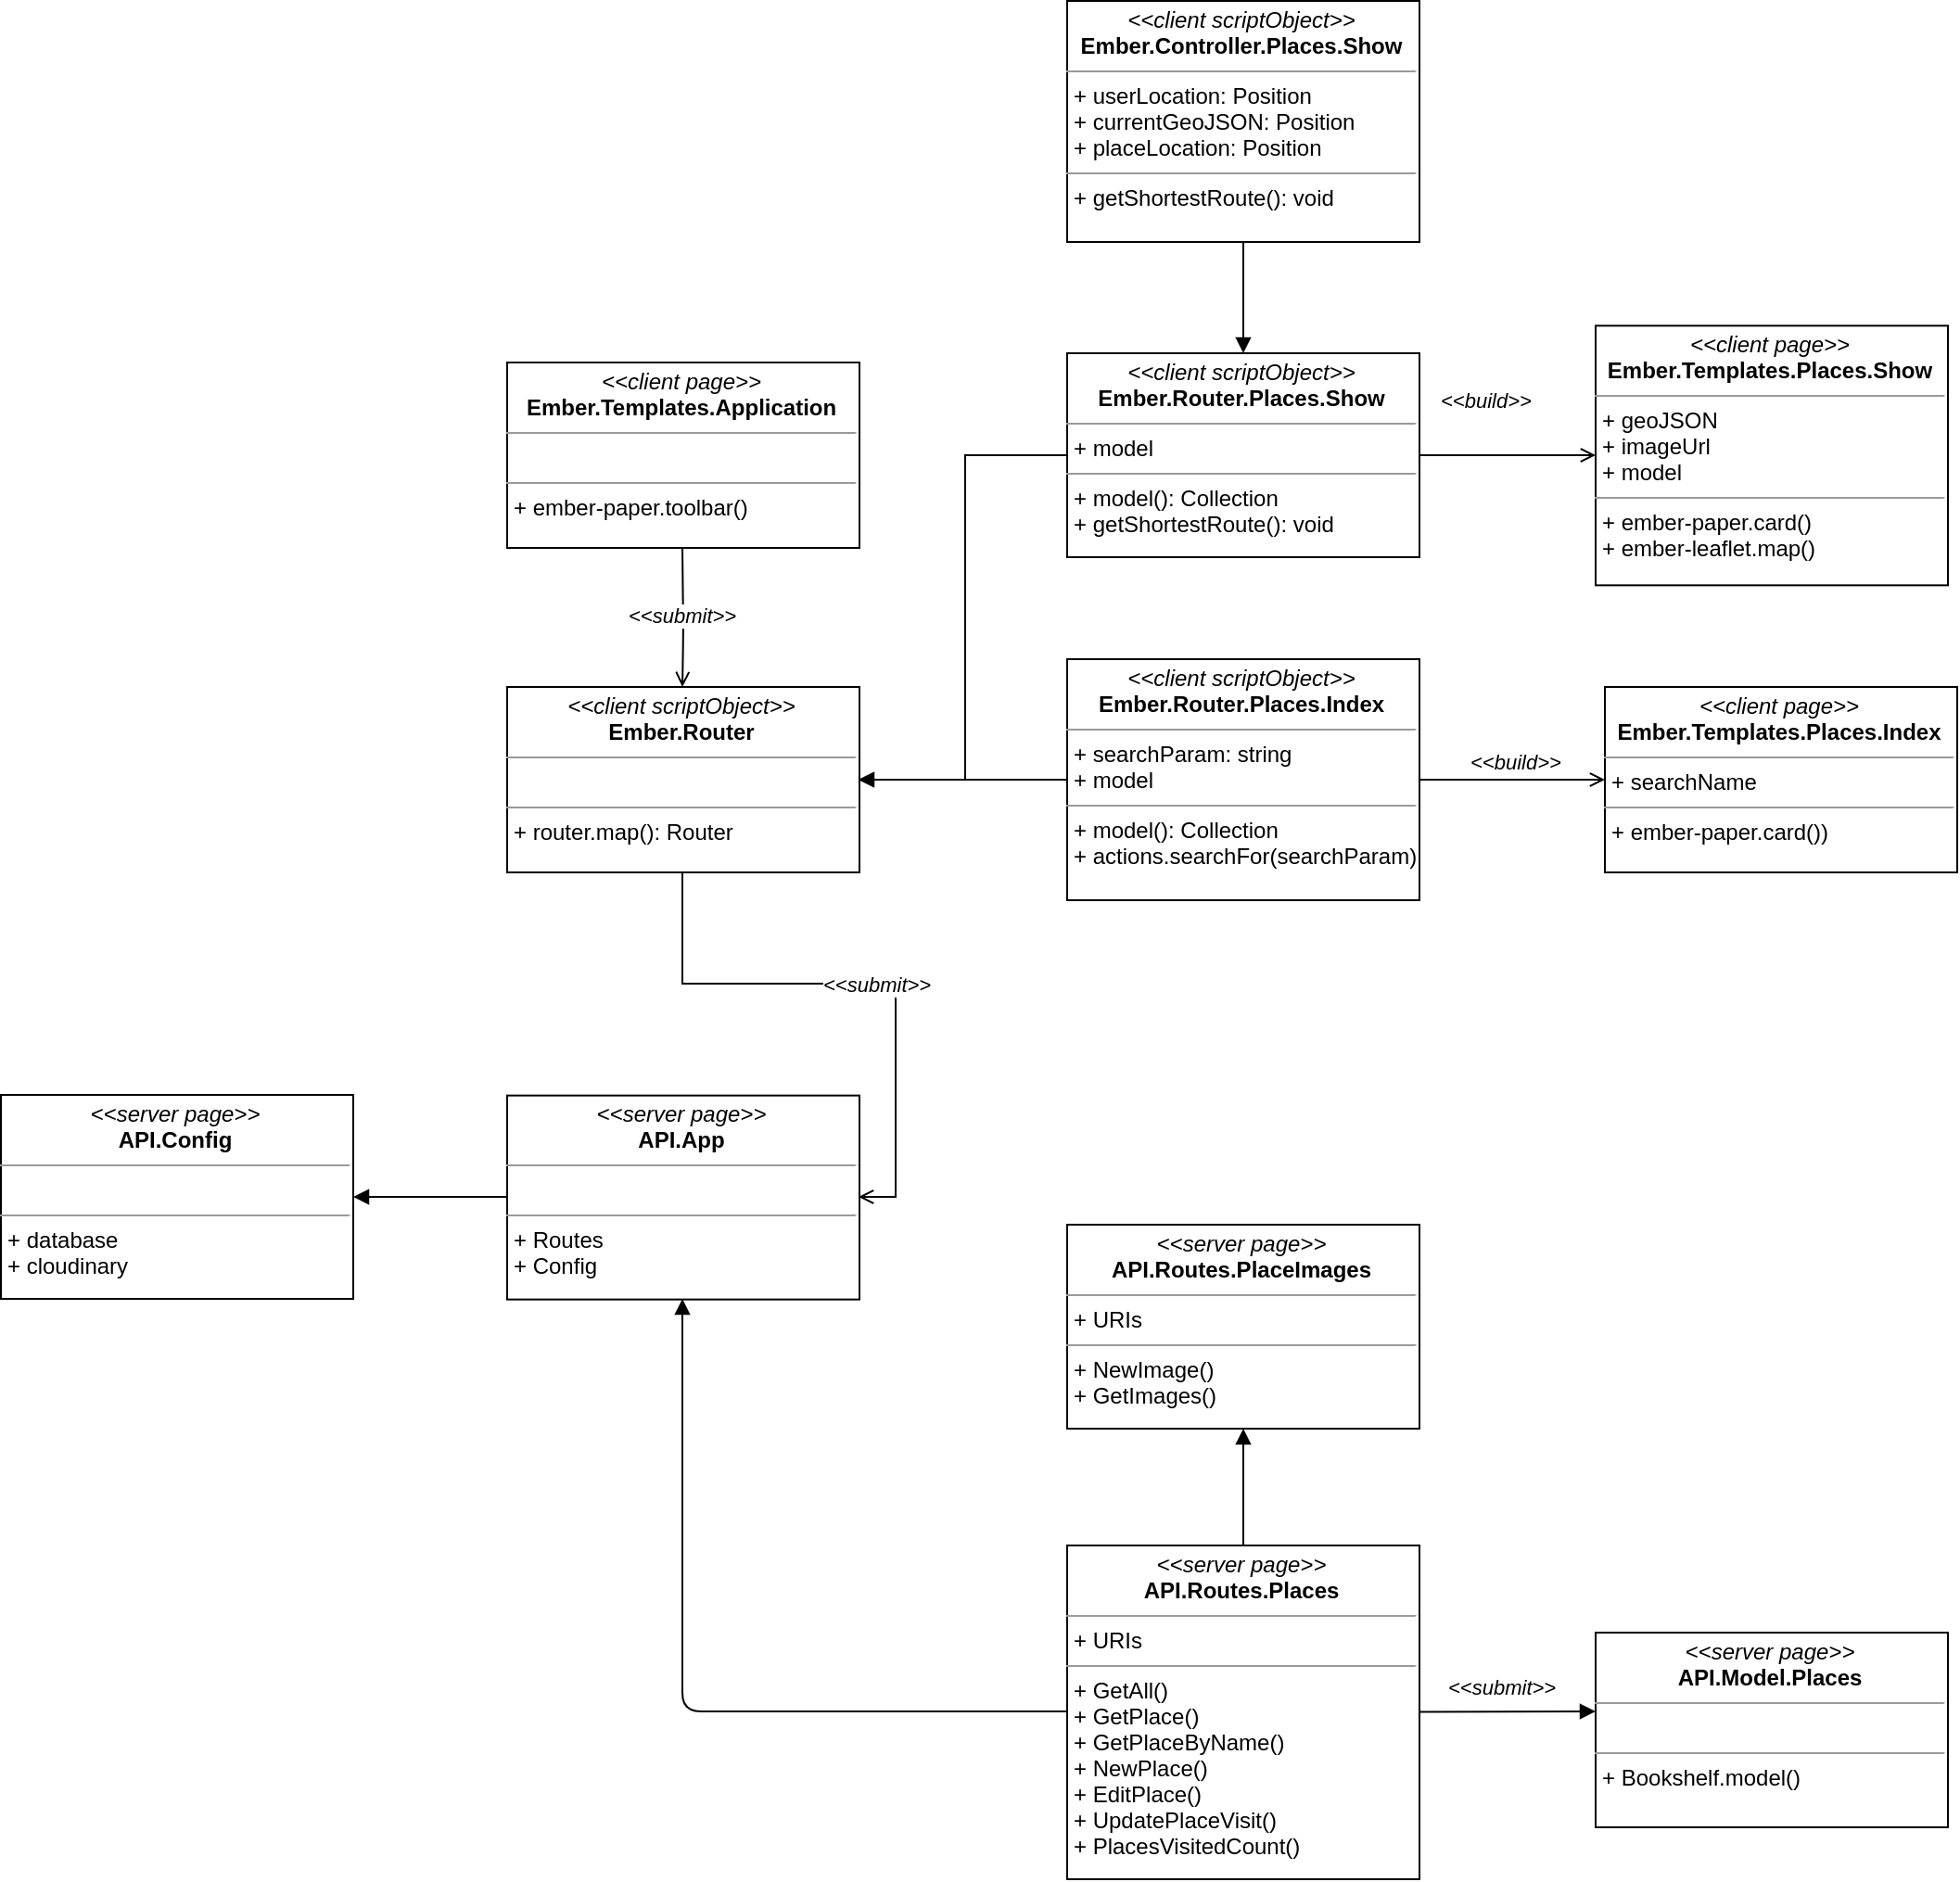
\includegraphics[width=0.9\textwidth]{diagramas/clases_lugares}
\end{center}
\caption{Diagrama de Clases: Lugares}
\label{fig:clases_lugares}
\caption*{Fuente: Elaboración propia}
\end{figure}


\end{itemize}
